\chapter{Laboratorio 3}
\section{Introduzione}
In questa esperienza di laboratorio, è stato analizzato il circuito di amplificazione \textit{common emitter amplifier} con degenerazione di emettitore, nella versione con alimentazione positiva e negativa e nella versione single-ended (\Fig\ref{fig:commonemitter}).
\begin{figure}[h!]
	\centering
	A
	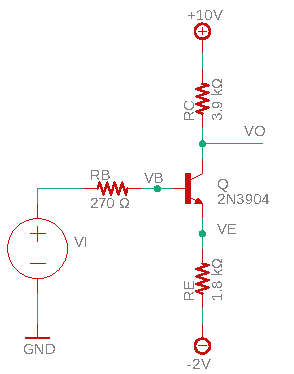
\includegraphics[width=0.4\linewidth]{./OtherFiles/Laboratorio 3/common emitter}
	B
	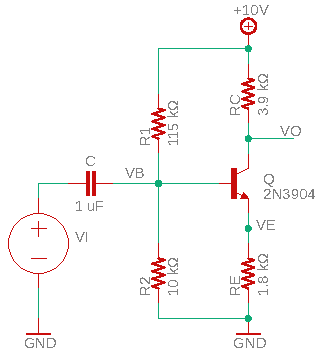
\includegraphics[width=0.4\linewidth]{./OtherFiles/Laboratorio 3/common emitter_se}
	\caption{Schematico del circuito common emitter con degenerazione di emettitore nella versione con alimentazione doppia (A) e singola (B).}
	\label{fig:commonemitter}
\end{figure}

\todo{inserire spiegazione del perchè degenerazione}

\section{Common emitter amplifier: punto di lavoro}
Prima di procedere alla realizzazione dei circuito analizziamone il punto di lavoro.

Consideriamo prima la versione con alimentazione doppia. Supponiamo il transistor in regione attiva diretta, con corrente di base nulla. Allora la tensione al nodo V\sub{B} sarà nulla (corrente nella resistenza R\sub{B} nulla). Allora, ricordando che $V_{BE}=\SI{-0.7}{\volt}$, si deriva che $V_E=\SI{-0.7}{\volt}$. Per cui, la corrente che attraversa la resistenza R\sub{E} è pari a (legge di Ohm) $I_E=\frac{V_E-(\SI{-2}{\volt})}{R_E}$. Dal bilancio di correnti nel transistor, si ricava che $I_C+I_B=I_E$. Dal momento che la corrente di base è considerata nulla, otteniamo che $I_C=I_E$. Ricaviamo poi V\sub{o} tramite legge di Ohm: $I_C=\frac{\SI{10}{\volt}-V_o}{R_C}$, da cui $V_o= \SI{10}{\volt}-R_C*I_C$. Inoltre, ricordiamo che $g_m=\frac{I_C^*}{\phi_T}$, con $I_C^*$ corrente di collettore stazionaria e $\phi_T\simeq\SI{26}{\milli\volt}$. Inoltre, sarà importante verificare che V\sub{BE} sia positiva, in modo da confermare l'ipotesi che il transistor si trova in regione attiva diretta.
\begin{figure}[h!]
	\centering
	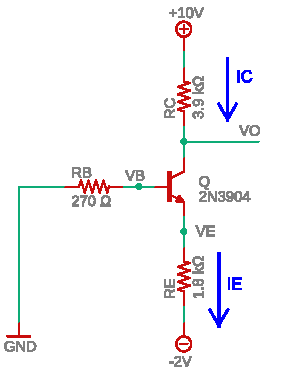
\includegraphics[width=0.4\linewidth]{./OtherFiles/Laboratorio 3/common emitter-punto di lavoro-printout}
	\caption{Analisi del punto di lavoro del circuito common emitter amplifier con alimentazione positiva e negativa.}
	\label{fig:commonemitter_DC}
\end{figure}

Sostituendo i valori dei componenti utilizzati nel circuito otteniamo i seguenti valori, che saranno da confrontare con quelli misurati sul circuito reale:
\begin{table}[h!]
	\centering
	\begin{tabular}{c|c|c|c|c|c|c}
		\hline
		V\sub{B} [V] & V\sub{E} [V] & V\sub{O} [V] & I\sub{B} [A] & I\sub{E} [mA] & I\sub{C} [mA] & g\sub{m} [A/V]\\ \hline
		0 & -0.7 & 7.183  & 0 & 0.7222 & 0.7222 & 0.0277 \\ \hline
	\end{tabular}
\end{table}
\todo{inserire tabella nel laboratorio 2}

Procediamo ora con l'analisi del punto di lavoro del circuito \textit{common emitter amplifier}, nella versione con alimentazione singola (\Fig\ref{fig:commonemitter_se_DC}).
\begin{figure}[h!]
	\centering
	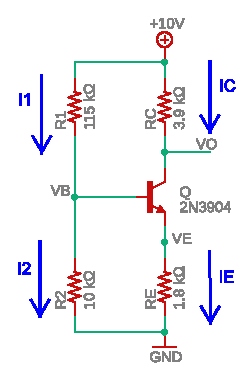
\includegraphics[width=0.4\linewidth]{./OtherFiles/Laboratorio 3/common emitter_se-punto di lavoro-printout}
	\caption{Analisi del punto di lavoro del circuito common emitter amplifier con alimentazione singola.}
	\label{fig:commonemitter_se_DC}
\end{figure}
Supponendo che la corrente di base sia zero (ossia che $\beta_Q\to\infty$), da un bilancio di corrente al nodi V\sub{B} e nel transistor, otteniamo che $I_1=I_2$ e $I_C=I_E$. Si noti che il condensatore è stato considerato come un circuito aperto nell'analisi DC. Infatti, il suo ruolo è quello di disaccoppiare in continua il circuito, in modo che la tensione imposta dal partitore di tensione formato da R\sub{1} e R\sub{2} non sia portata a massa dal generatore V\sub{i}. Infatti, come già discusso in precedenza nell'analisi dell'emitter follower single-ended, le resistenze R\sub{1} e R\sub{2} hanno il compito di alzare la tensione nel nodo V\sub{B}, in modo da mantenere il transistor in zona attiva diretta.

Ricaviamo quindi la tensione V\sub{B} utilizzando la legge di Ohm:
\begin{equation}
	\begin{split}
		I=I_1&=I_2 \\
		\frac{\SI{10}{\volt}-V_B}{R_1}&=\frac{V_B-\SI{0}{\volt}}{R_2} \\
		V_B&=\frac{R_2}{R_1+R_2}*\SI{10}{\volt}
	\end{split}
\end{equation}

La tensione al nodo V\sub{E} è $V_{BE}=V_B-V_E=\SI{0.7}{\volt}$ (transistor in zona attiva diretta), da cui $V_E=V_B-\SI{0.7}{\volt}$. Conoscendo V\sub{E} è ora possibile calcolare la corrente I\sub{E} e I\sub{C} tramite la legge di Ohm: $I_E=I_C=\frac{V_E-\SI{0}{\volt}}{R_E}$. 
Infine, la tensione nel nodo V\sub{O} sarà $V_O=\SI{10}{\volt}-I_C*R*C$. Si dovrà inoltre verificare che la tensione V\sub{CE} sia maggiore di zero.

Sostituendo i valori dei componenti utilizzati nel circuito otteniamo i seguenti valori, che saranno da confrontare con quelli misurati sul circuito reale:
\begin{table}[h!]
	\centering
	\begin{tabular}{c|c|c|c|c|c|c}
		\hline
		V\sub{B} [mV] & V\sub{E} [mV] & V\sub{O} [V] & I\sub{B} [A] & I\sub{E} [mA] & I\sub{C} [mA] & g\sub{m} [A/V]\\ \hline
		800 & 100 & 9.783 & 0 & 0.055 & 0.055 & 0.0021 \\ \hline
	\end{tabular}
\end{table}

\section{Common emitter amplifier: analisi per piccolo segnale}
Analizziamo ora il circuito sotto l'ipotesi di piccolo segnale, utilizzando il modello per piccolo segnale del transistor e spegnendo i generatori di grandezze continue.

Considerando il circuito a emettitore comune con alimentazione doppia si ottiene il circuito in figura \ref{fig:commonemitter_AC}.
\begin{figure}[h!]
	\centering
	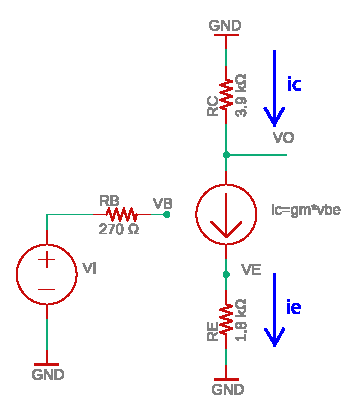
\includegraphics[width=0.4\linewidth]{./OtherFiles/Laboratorio 3/common emitter-piccolo segnale-printout}
	\caption{Analisi per piccolo segnale del circuito common emitter amplifier con alimentazione positiva e negativa.}
	\label{fig:commonemitter_AC}
\end{figure}

Dal momento che nella resistenza R\sub{B} non passa corrente, $v_b=v_i$. Inoltre si possono ricavare le seguenti equazioni (utilizzando legge di Ohm e bilanci di corrente):
\begin{equation}
	\begin{cases}
		i_c=\frac{-v_o}{R_C} \\
		i_c=gm*v_{be}=gm*v_{ie} \\
		i_c=\frac{v_e}{R_E} \\
		i_e=i_c
	\end{cases}
\end{equation}
Risolvendo il sistema, è possibile calcolare la funzione di trasferimento del circuito:
\begin{equation}
	\frac{v_o}{v_i}=-\frac{R_C*g_m}{1+R_E*g_m}\;\underset{g_m*R_E\gg 1}{\simeq}\;-\frac{R_C}{R_E}.
\end{equation}
Il guadagno del circuito è quindi determinato dal rapporto tra la resistenza di collettore e quella di emettitore. Inoltre, la presenza di un segno meno nella funzione di trasferimento indica che il circuito introduce uno sfasamento di \SI{-90}{\degree} tra il segnale in ingresso e quello in uscita (amplificatore invertente). 

L'analisi di piccolo segnale della versione con singola alimentazione è identica a quella presentata precedentemente sotto l'ipotesi che $C\to\infty$, ossia che il condensatore si comporti come un corto circuito per frequenze del segnale sufficientemente alte. Sotto questa ipotesi semplificativa, $v_b=v_i$. Con la risoluzione del medesimo sistema di equazioni si determina che il guadagno è $\frac{v_o}{v_i}\simeq-\frac{R_C}{R_E}.$
\begin{figure}[h!]
	\centering
	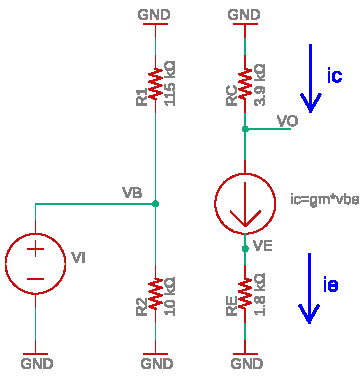
\includegraphics[width=0.4\linewidth]{./OtherFiles/Laboratorio 3/common emitter_se-piccolo segnale-printout}
	\caption{Analisi per piccolo segnale del circuito common emitter amplifier con alimentazione singola.}
	\label{fig:commonemitter_se_AC}
\end{figure}

Sostituendo i valori delle resistenze da utilizzare nei nostri circuiti ci aspettiamo un guadagno di:
\begin{equation}
	\frac{v_o}{v_i}=-\frac{\SI{3.9}{\kilo\ohm}}{\SI{1.8}{\kilo\ohm}}\simeq -2.17.
\end{equation}

\section{Componenti e misure}
I due circuiti sono stati realizzati in laboratorio (\Fig\ref{fig:commonemitter_circuito}), utilizzando i seguenti componenti:
\begin{figure}[h!]
	\centering
	A)
	
	\includegraphics[width=0.6\linewidth]{./ImageFiles/Laboratorio 3/IMG\_20220524\_110713_2}
	
	B)
	
	\includegraphics[width=0.6\linewidth]{./ImageFiles/Laboratorio 3/IMG\_20220524\_122237\_2}
	\caption{Foto del circuito realizzato in laboratorio nella versione con doppia (A) e singola (B) alimentazione.}
	\label{fig:commonemitter_circuito}
\end{figure}

\todo{da completare componenti}
\begin{itemize}
	\item transistor 2N3904;
	\item una resistenza da \SI{270}{\ohm} per realizzare la resistenza R\sub{B};
	\item due resistenze rispettivamente da R\sub{E1}=\SI{1.5}{\ohm} e R\sub{E1}2=\SI{1.8}{\ohm} connesse in parallelo per realizzare la resistenza R\sub{E}.
\end{itemize}
Inoltre, sono state utilizzate i seguenti strumenti:
\begin{itemize}
	\item alimentatore da banco con tensione positiva \SI{10}{\volt}, tensione negativa \SI{-10}{\volt} e limite in corrente di \SI{50}{\milli\ampere};
	\item oscilloscopio a due canali;
	\item generatore di forme d'onda;
	\item multimetro da banco.
\end{itemize}
